\section{Types and Operators}

\begin{frame}
    \frametitle{The Python interpreter}

    \begin{itemize}
        \item Python is an interpreted language.
        \item Commands are executed through the Python interpreter.
              \begin{itemize}
                  \item The interpreter receives a command, evaluates that command, and reports the result of the command.
              \end{itemize}
        \item A programmer defines a series of commands in advance and saves those commands in a text file known as source code or a script.
        \item For Python, source code is conventionally stored in a file named with the .py suffix (e.g., demo.py).

    \end{itemize}

\end{frame}

\begin{frame}[fragile]
    \frametitle{An example program}

    \begin{minted}{python}            
        print("Welcome to the GPA calculator.")
        print("Please enter all your letter grades, one per line")
        print("Enter a blank line to designate the end.")
        # map from letter grade to point value
        points = {
            "A+": 4.0,  "A": 4.0, "A-": 3.67, 
            "B+": 3.33, "B": 3.0, "B-": 2.67, 
            "C+": 2.33, "C": 2.0, "C-": 1.67, 
            "D+": 1.33, "D": 1.0, "F": 0.0
        }
        num_courses = 0
        total_points = 0
        done = False
    \end{minted}
\end{frame}

\begin{frame}[fragile]
    \frametitle{An example program cont.}

    \begin{minted}[firstnumber=14]{python}
        while not done:
            grade = input()                 # read line from user
            if grade == "":                 # empty line was entered
                done = True
            elif grade not in points:       # unrecognized grade entered
                print(f"Unknown grade {grade} being ignored")
            else:
                num_courses += 1
                total_points += points[grade]
        if num_courses > 0:                 # avoid division by zero
        print(f"Your GRA is {total_points / num_courses:.2f}")
    \end{minted}

\end{frame}

\begin{frame}
    \frametitle{Objects in Python}

    \begin{itemize}
        \item Python is an object-oriented language and classes form the basis for all data types.
        \item Python's built-in classes:
              \begin{itemize}
                  \item the \mintinline{python}|int| class for integers,
                  \item the \mintinline{python}|float| class for floating-point values,
                  \item the \mintinline{python}|str| class for character strings.
              \end{itemize}
    \end{itemize}

\end{frame}

\begin{frame}[fragile]
    \frametitle{Identifiers, objects, and the assignment statement}

    \begin{itemize}
        \item The most important of all Python commands is an assignment statement:
              \begin{center}
                  \mintinline{python}|temperature = 98.6|
              \end{center}
        \item This command establishes temperature as an identifier (also known as a name), and then associates it with the object expressed on the right-hand side of the equal sign, in this case a floating-point object with value 98.6.

    \end{itemize}

    \begin{figure}
        \centering
        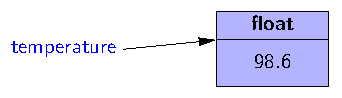
\includegraphics{../images/figure-1.1.pdf}
    \end{figure}

\end{frame}

\begin{frame}[fragile]
    \frametitle{Identifiers}

    \begin{itemize}
        \item Identifiers in Python are case-sensitive, so \mintinline{python}|temperature| and \mintinline{python}|Temperature| are distinct names.
        \item Identifiers can be composed of almost any combination of letters, numerals, and underscore characters.
        \item An identifier cannot begin with a numeral and that there are 35 specially \href{https://docs.python.org/3/reference/lexical_analysis.html#keywords}{reserved words} that cannot be used as identifiers.
    \end{itemize}

\end{frame}


\begin{frame}
    \frametitle{Types}

    \begin{itemize}
        \item Python is a dynamically typed language, as there is no advance declaration associating an identifier with a particular data type.
        \item An identifier can be associated with any type of object, and it can later be reassigned to another object of the same (or different) type.
        \item Although an identifier has no declared type, the object to which it refers has a definite type. In our first example, the characters 98.6 are recognized as a floating-point literal, and thus the identifier temperature is associated with an instance of the float class having that value.

    \end{itemize}

\end{frame}

\begin{frame}
    \frametitle{Objects}

    \begin{itemize}
        \item The process of creating a new instance of a class is known as \emph{instantiation}.
        \item To instantiate an object we usually invoke the constructor of a class: \mintinline{python}|w = Widget()|
        \item This is assuming that the constructor does not require any parameters.
        \item If the constructor does require parameters, we might use a syntax such as \mintinline{python}|w = Widget(a, b, c)|
        \item Many of Python's built-in classes a literal form for designating new instances. For example, the command \mintinline{python}|temperature = 98.6|, results in the creation of a new instance of the float class.

    \end{itemize}

\end{frame}

\begin{frame}
    \frametitle{Calling methods}

    \begin{itemize}
        \item Python supports functions a syntax such as \mintinline{python}|sorted(data)|, in which case data is a parameter sent to the function.
        \item Python's classes may also define one or more methods (also known as member functions), which are invoked on a specific instance of a class using the dot (``\mintinline{python}|.|'') operator.
        \item For example, Python's list class has a method named sort that can be invoked with a syntax such as \mintinline{python}|data.sort()|.
        \item This particular method rearranges the contents of the list so that they are sorted.

    \end{itemize}

\end{frame}

\begin{frame}
    \frametitle{Built-In classes}

    % Table generated by Excel2LaTeX from sheet 'Sheet1'
    \begin{table}
        \footnotesize
        \centering
        % \caption{Add caption}
        \begin{tabular}{llc}
            \toprule
            \textbf{Class}                 & \textbf{Description}                 & \multicolumn{1}{l}{\textbf{Immutable?}} \\
            \midrule
            \mintinline{python}|bool|      & Boolean value                        & \checkmark                              \\
            \mintinline{python}|int|       & integer (arbitrary magnitude)        & \checkmark                              \\
            \mintinline{python}|float|     & floating-point number                & \checkmark                              \\
            \mintinline{python}|list|      & mutable sequence of objects          &                                         \\
            \mintinline{python}|tuple|     & immutable sequence of objects        & \checkmark                              \\
            \mintinline{python}|str|       & character string                     & \checkmark                              \\
            \mintinline{python}|set|       & unordered set of distinct objects    &                                         \\
            \mintinline{python}|frozenset| & immutable form of set class          & \checkmark                              \\
            \mintinline{python}|dict|      & associative mapping (aka dictionary) &                                         \\
            \bottomrule
        \end{tabular}%
        % \label{tab:addlabel}%
    \end{table}%

    \begin{itemize}
        \item A class is \emph{immutable} if each object of that class has a fixed value upon instantiation that cannot subsequently be changed. For example, the \mintinline{python}|float| class is immutable.
    \end{itemize}

\end{frame}

\begin{frame}
    \frametitle{The \mintinline{python}|bool| class}

    \begin{itemize}
        \item The \mintinline{python}|bool| class is used for logical (Boolean) values, and the only two instances of that class are expressed as the literals: \mintinline{python}|True| and  \mintinline{python}|False|
        \item The default constructor, \mintinline{python}|bool()|, returns \mintinline{python}|False|.
        \item Python allows the creation of a Boolean value from a nonboolean type using the syntax \mintinline{python}|bool(foo)| for value \mintinline{python}|foo|. The interpretation depends upon the type of the parameter.
              \begin{itemize}
                  \item Numbers evaluate to \mintinline{python}|False| if zero, and \mintinline{python}|True| if nonzero.
                  \item Sequences and other container types, such as strings and lists, evaluate to \mintinline{python}|False| if empty and \mintinline{python}|True| if nonempty.
              \end{itemize}
    \end{itemize}

\end{frame}

\begin{frame}
    \frametitle{The \mintinline{python}|int| Class}

    \begin{itemize}
        \item The \mintinline{python}|int| class is designed to represent integer values with arbitrary magnitude.
              \begin{itemize}
                  \item Python automatically chooses the internal representation for an integer based upon the magnitude of its value.
              \end{itemize}
        \item The integer constructor, \mintinline{python}|int()|, returns \mintinline{python}|0| by default.
        \item This constructor can also construct an integer value based upon an existing value of another type.
              \begin{itemize}
                  \item For example, if \mintinline{python}|f| represents a floating-point value, the syntax \mintinline{python}|int(f)| produces the truncated value of \mintinline{python}|f|. For example, \mintinline{python}|int(3.14)| produces the value \mintinline{python}|3|, while \mintinline{python}|int(-3.9)| produces the value \mintinline{python}|-3|.
                  \item The constructor can also be used to parse a string that represents an integer. For example, the expression \mintinline{python}|int("137")| produces the integer value \mintinline{python}|137|.
              \end{itemize}
    \end{itemize}

\end{frame}

\begin{frame}
    \frametitle{The \mintinline{python}|float| Class}

    \begin{itemize}
        \item The \mintinline{python}|float| class is the floating-point type in Python.
              \begin{itemize}
                  \item The floating-point equivalent of an integral number, \mintinline{python}|2|, can be expressed directly as \mintinline{python}|2.0|.
                  \item One other form of literal for floating-point values uses scientific notation. For example, the literal \mintinline{python}|6.022e23| represents the mathematical value \(6.022\times10^{23}\).
              \end{itemize}
        \item The constructor \mintinline{python}|float()| returns \mintinline{python}|0.0|.
        \item When given a parameter, the constructor, \mintinline{python}|float|, returns the equivalent floating-point value.
              \begin{itemize}
                  \item \mintinline{python}|float(2)| returns the floating-point value \mintinline{python}|2.0|
                  \item \mintinline{python}|float("3.14"|) returns \mintinline{python}|3.14|
              \end{itemize}
    \end{itemize}

\end{frame}

\begin{frame}
    \frametitle{The \mintinline{python}|list| Class}

    \begin{itemize}
        \item A \mintinline{python}|list| instance stores a sequence of objects, that is, a sequence of references (or pointers) to objects in the list.
        \item Elements of a list may be arbitrary objects (including the \mintinline{python}|None| object).
        \item Lists are array-based sequences and a list of length \mintinline{python}|n| has elements indexed from \mintinline{python}|0| to \mintinline{python}|n-1| inclusive.
        \item Lists have the ability to dynamically expand and contract their capacities as needed.
        \item Python uses the characters \mintinline{python}|[ ]| as delimiters for a list literal.
              \begin{itemize}
                  \item \mintinline{python}|[ ]| is an empty list.
                  \item \mintinline{python}|["red", "green", "blue"]| is a list containing three string instances.
              \end{itemize}
        \item The \mintinline{python}|list()| constructor produces an empty list by default.
        \item The list constructor will accept any iterable parameter.
              \begin{itemize}
                  \item \mintinline{python}|list("hello")| produces a list of individual characters, \mintinline{python}|['h', 'e', 'l', 'l', 'o']|.
              \end{itemize}

    \end{itemize}

\end{frame}

\begin{frame}
    \frametitle{The \mintinline{python}|tuple| Class}

    \begin{itemize}
        \item The \mintinline{python}|tuple| class provides an immutable (unchangeable) version of a sequence, which allows instances to have an internal representation that may be more streamlined than that of a list. Parentheses delimit a tuple.
              \begin{itemize}
                  \item The empty tuple is \mintinline{python}|()|
              \end{itemize}
        \item To express a tuple of length one as a literal, a comma must be placed after the element, but within the parentheses.
              \begin{itemize}
                  \item For example, \mintinline{python}|(17,)| is a one-element tuple.
              \end{itemize}

    \end{itemize}

\end{frame}

\begin{frame}[fragile]
    \frametitle{The \mintinline{python}|str| Class}

    \begin{itemize}
        \item String literals can be enclosed in single quotes, as in \mintinline{python}|'hello'|, or double quotes, as in \mintinline{python}|"hello"|.
        \item A string can also begin and end with three single or double quotes, if it contains newlines in it. For example
              \vspace{\baselineskip}
              \begin{minted}{python}
                print("""Welcome to the GPA calculator.
                Please enter all your letter grades, one per line.
                Enter a blank line to designate the end.""")
              \end{minted}
    \end{itemize}
\end{frame}

\begin{frame}
    \frametitle{The \mintinline{python}|set| Class}

    \begin{itemize}
        \item Python's \mintinline{python}|set| class represents a set, namely a collection of elements, without duplicates, and without an inherent order to those elements.
        \item Only instances of immutable types can be added to a Python \mintinline{python}|set|. Therefore, objects such as integers, floating-point numbers, and character strings are eligible to be elements of a set.
              \begin{itemize}
                  \item The \mintinline{python}|frozenset| class is an immutable form of the set type, itself.
              \end{itemize}
        \item Python uses curly braces \{ and \} as delimiters for a set
              \begin{itemize}
                  \item For example, as \{\mintinline{python}|17|\} or \{\mintinline{python}|'red', 'green', 'blue'|\}
                  \item  The exception to this rule is that { } does not represent an empty set. Instead, the constructor \mintinline{python}|set()| returns an empty set.
              \end{itemize}

    \end{itemize}
\end{frame}

\begin{frame}
    \frametitle{The \mintinline{python}|dict| Class}

    \begin{itemize}
        \item  Python's \mintinline{python}|dict| class represents a dictionary, or mapping, from a set of distinct keys to associated values.
        \item Python implements a \mintinline{python}|dict| using an almost identical approach to that of a set, but with storage of the associated values.
              \begin{itemize}
                  \item The literal form \{ \} produces an empty dictionary.
              \end{itemize}
        \item A nonempty dictionary is expressed using a comma-separated series of key:value pairs. For example, the dictionary \{\mintinline{python}|'ga' : 'Irish', 'de' : 'German'|\} maps \mintinline{python}|'ga'| to \mintinline{python}|'Irish'| and \mintinline{python}|'de'| to \mintinline{python}|'German'|.
        \item Alternatively, the constructor accepts a sequence of key-value pairs as a parameter, as in \mintinline{python}|dict(pairs)| with pairs = \mintinline{python}|[('ga', 'Irish'), ('de', 'German')]|.
    \end{itemize}

\end{frame}

\begin{frame}
    \frametitle{Expressions and operators}

    \begin{itemize}
        \item Existing values can be combined into expressions using special symbols and keywords known as operators.
        \item The semantics of an operator depends upon the type of its operands.
        \item For example, when a and b are numbers, the syntax \mintinline{python}|a + b| indicates addition, while if \mintinline{python}|a| and \mintinline{python}|b| are strings, the operator \mintinline{python}|+| indicates concatenation.

    \end{itemize}

\end{frame}

\begin{frame}
    \frametitle{Logical operators}

    \begin{itemize}
        \item Python supports the following keyword operators for Boolean values: \mintinline{python}|not|, \mintinline{python}|and| and \mintinline{python}|or|
        \item The \mintinline{python}|and| and \mintinline{python}|or| operators short-circuit, in that they do not evaluate the second operand if the result can be determined based on the value of the first operand.

    \end{itemize}

\end{frame}

\begin{frame}
    \frametitle{Equality operators}

    \begin{itemize}
        \item Python supports the following operators to test two notions of equality: \mintinline{python}|is|, \mintinline{python}|is not|, \mintinline{python}|==| and \mintinline{python}|!=|
        \item The expression, \mintinline{python}|a is b|, evaluates to \mintinline{python}|True|, precisely when identifiers \mintinline{python}|a| and \mintinline{python}|b| are aliases for the same object.
        \item The expression \mintinline{python}|a == b| tests a more general notion of equivalence.

    \end{itemize}

\end{frame}

\begin{frame}
    \frametitle{Comparison operators}

    \begin{itemize}
        \item Data types may define a natural order via the following operators: \mintinline{python}|>|, \mintinline{python}|>=|, \mintinline{python}|<|, and \mintinline{python}|<=|
        \item These operators have expected behavior for numeric types, and are defined lexicographically, and case-sensitively, for strings.
    \end{itemize}

\end{frame}

\begin{frame}
    \frametitle{Arithmetic operators}

    \begin{itemize}
        \item Python supports the following arithmetic operators: \mintinline{python}|+|, \mintinline{python}|-|, \mintinline{python}|*|, \mintinline{python}|/|, \mintinline{python}|//|, \footnotesize{\%}.
        \item For addition, subtraction, and multiplication, if both operands have type \mintinline{python}|int|, then the result is an \mintinline{python}|int|; if one or both operands have type \mintinline{python}|float|, the result is a \mintinline{python}|float|.
        \item True division is always of type \mintinline{python}|float|, integer division is always \mintinline{python}|int| (with the result truncated)

    \end{itemize}

\end{frame}

\begin{frame}
    \frametitle{Bitwise operators}

    \begin{itemize}
        \item Python provides the following bitwise operators for integers:
              % Table generated by Excel2LaTeX from sheet 'Sheet1'
              \begin{table}[htbp]
                  \centering
                  % \caption{Add caption}
                  \begin{tabular}{ll}
                      \mintinline{python}|~|  & bitwise complement (prefix unary operator) \\
                      \&                      & bitwise and                                \\
                      \mintinline{python}|||  & bitwise or                                 \\
                      \mintinline{python}|^|  & bitwise exclusive-or                       \\
                      \mintinline{python}|<<| & shift bits left, filling in with zeros     \\
                      \mintinline{python}|>>| & shift bits right, filling in with sign bit \\
                  \end{tabular}%
                  % \label{tab:addlabel}%
              \end{table}%

    \end{itemize}

\end{frame}

\begin{frame}
    \frametitle{Sequence operators}

    \begin{itemize}
        \item Each of Python's built-in sequence types (\mintinline{python}|str|, \mintinline{python}|tuple|, and \mintinline{python}|list|) support the following operator syntaxes:
              % Table generated by Excel2LaTeX from sheet 'Sheet1'
              \begin{table}[htbp]
                  \centering
                  %   \caption{Add caption}
                  \begin{tabular}{rl}
                      \mintinline{python}|s[j]|               & element at index $j$                                                                            \\
                      \mintinline{python}|s[start:stop]|      & slice including indices                                                                         \\
                      \mintinline{python}|s[start:stop:step]| & slice including indices \mintinline{python}|start|, \mintinline{python}|start + step|,          \\
                                                              & \mintinline{python}|start + 2 * step|, … , up to but not equalling to \mintinline{python}|stop| \\
                      \mintinline{python}|s + t|              & concatenation of sequences                                                                      \\
                      \mintinline{python}|k * s|              & shorthand for \mintinline{python}|s + s +| … ($k$ times)                                        \\
                      \mintinline{python}|val in s|           & containment check                                                                               \\
                      \mintinline{python}|val not in s|       & non-containment check                                                                           \\
                  \end{tabular}%
                  %   \label{tab:addlabel}%
              \end{table}%

    \end{itemize}

\end{frame}

\begin{frame}
    \frametitle{Sequence comparisons}

    \begin{itemize}
        \item Sequences define comparison operations based on lexicographic order, performing an element by element comparison until the first difference is found.
        \item For example, \mintinline{python}|[5, 6, 9] < [5, 7]| because of the entries at index 1.
              % Table generated by Excel2LaTeX from sheet 'Sheet1'
              \begin{table}[htbp]
                  \centering
                  % \caption{Add caption}
                  \begin{tabular}{rl}
                      \mintinline{python}|s == t| & equivalent (element by element)            \\
                      \mintinline{python}|s != t| & not equivalent                             \\
                      \mintinline{python}|s < t|  & lexicographically less than                \\
                      \mintinline{python}|s <= t| & lexicographically less than or equal to    \\
                      \mintinline{python}|s > t|  & lexicographically greater than             \\
                      \mintinline{python}|s >= t| & lexicographically greater than or equal to \\
                  \end{tabular}%
                  % \label{tab:addlabel}%
              \end{table}%

    \end{itemize}

\end{frame}

\begin{frame}
    \frametitle{Operators for sets}

    \begin{itemize}
        \item Sets and frozensets support the following operators:
              % Table generated by Excel2LaTeX from sheet 'Sheet1'
              \begin{table}[htbp]
                  \centering
                  % \caption{Add caption}
                  \begin{tabular}{ll}
                      \mintinline{python}|key in s|            & containment check                                \\
                      \mintinline{python}|key not in s|        & non-containment check                            \\
                      \mintinline{python}|s1 == s2|            & s1 is equivalent to s2                           \\
                      \mintinline{python}|s1 != s2|            & s1 is not equivalent to s2                       \\
                      \mintinline{python}|s1 <= s2|            & s1 is subset of s2                               \\
                      \mintinline{python}|s1 < s2|             & s1 is proper subset of s2                        \\
                      \mintinline{python}|s1 >= s2|            & s1 is superset of s2                             \\
                      \mintinline{python}|s1 > s2|             & s1 is proper superset of s2                      \\
                      \footnotesize{s1}~~|~~\footnotesize{s2}  & the union of s1 and s2                           \\
                      \footnotesize{s1}~~\&~~\footnotesize{s2} & the intersection of s1 and s2                    \\
                      \mintinline{python}|s1 - s2|             & the set of elements in s1 but not s2             \\
                      \mintinline{python}|s1 ^ s2|             & the set of elements in precisely one of s1 or s2 \\
                  \end{tabular}%
                  % \label{tab:addlabel}%
              \end{table}%

    \end{itemize}

\end{frame}

\begin{frame}
    \frametitle{Operators for dictionaries}

    \begin{itemize}
        \item The supported operators for objects of type dict are as follows:
              % Table generated by Excel2LaTeX from sheet 'Sheet1'
              \begin{table}[htbp]
                  \centering
                  % \caption{Add caption}
                  \begin{tabular}{ll}
                      \mintinline{python}|d[key]|         & value associated with given key                    \\
                      \mintinline{python}|d[key] = value| & set (or reset) the value associate with given key  \\
                      \mintinline{python}|del d[key]|     & remove key and its associate value from dictionary \\
                      \mintinline{python}|key in d|       & containment check                                  \\
                      \mintinline{python}|key not in d|   & non-containment check                              \\
                      \mintinline{python}|d1 == d2|       & d1 is equivalent to d2                             \\
                      \mintinline{python}|d1 != d2|       & d1 is not equivalent to d2                         \\
                  \end{tabular}%
                  % \label{tab:addlabel}%
              \end{table}%

    \end{itemize}

\end{frame}

\begin{frame}
    \frametitle{Operator precedence}

    \begin{figure}
        \centering
        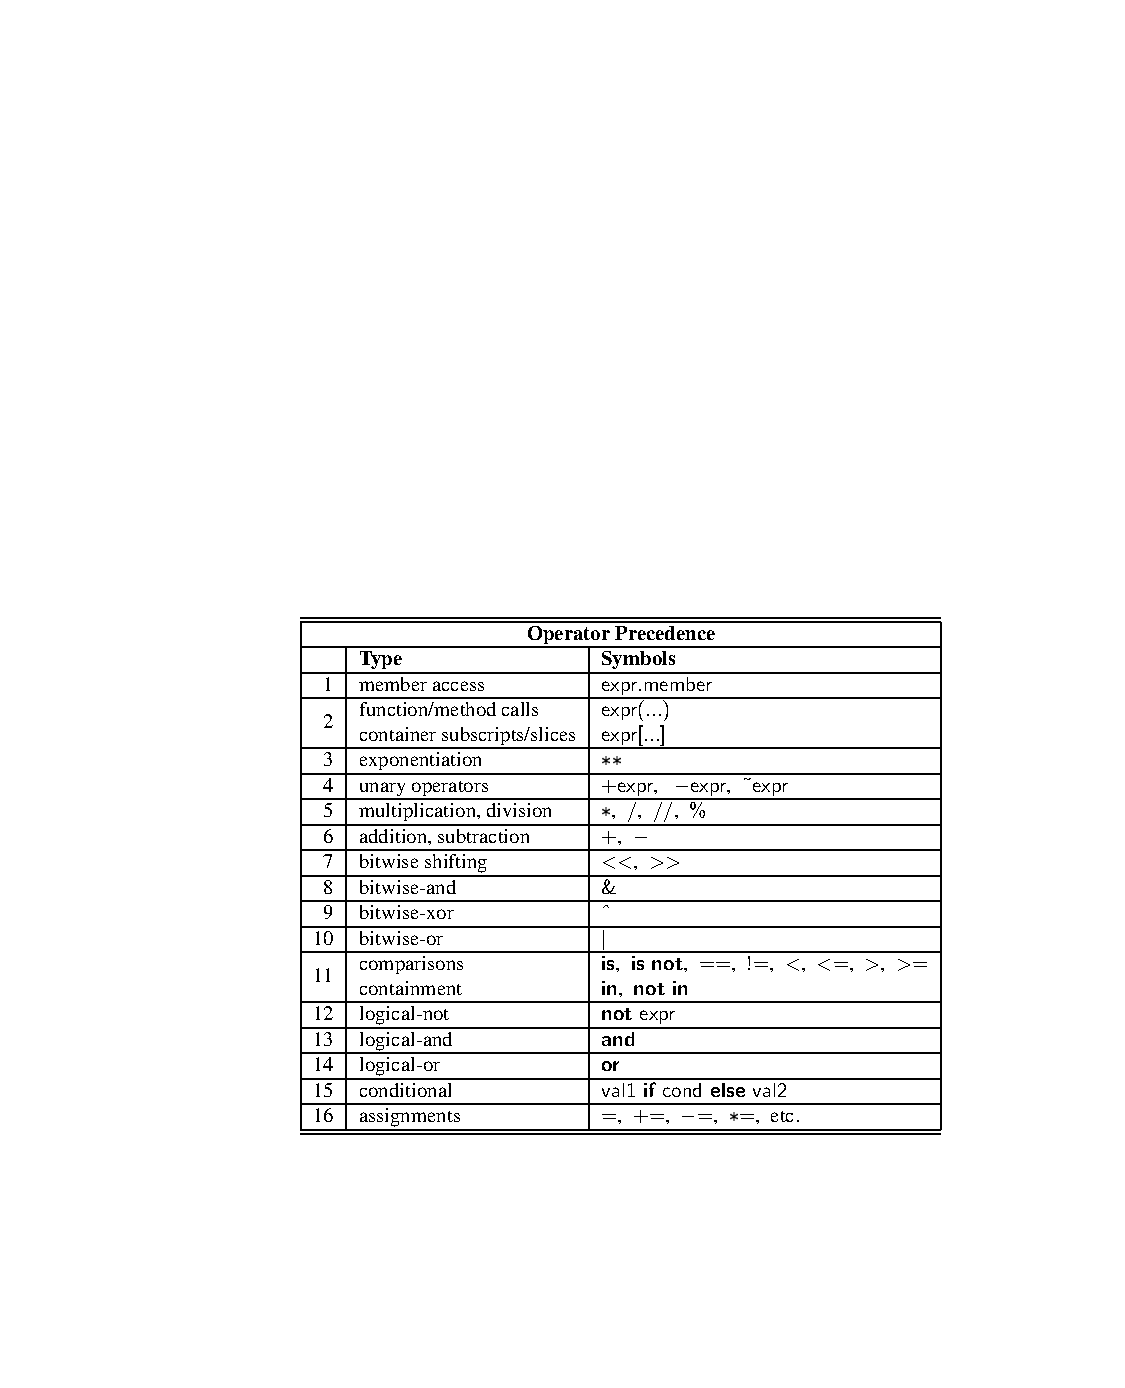
\includegraphics[height = \textheight]{../images/figure-1.9_operator_precedence.pdf}
    \end{figure}

\end{frame}

\section{}

